\chapter{Revue de littérature}
\label{chap:etat_art}
Ce chapitre inscrit le mémoire dans trois corpus complémentaires : la gouvernance documentaire et la numérisation de l'état civil en Afrique subsaharienne; les standards de description archivistique ; et les techniques de traitement automatique applicables aux documents manuscrits.

Il s'organise en cinq sections : les dynamiques institutionnelles de l'état civil, les registres manuscrits comme patrimoine documentaire, les standards descriptifs, les chaînes d'extraction sémantique et la frugalité computationnelle.

\section{État civil, gouvernance documentaire et dynamiques régionales de numérisation}

\subsection{Gouvernance documentaire publique et rôle archivistique de l'état civil}

La gouvernance documentaire désigne l'ensemble des politiques, responsabilités et procédures encadrant la création, la capture et la gestion des documents d'activité tout au long de leur cycle de vie.
Selon l'ISO 15489-1\string:2016, un \og record \fg{} est une information conservée comme preuve d'une activité ou d'une obligation légale \cite{iso2016-15489}.
Établi par une autorité compétente, l'acte d'état civil constitue ainsi une preuve officielle d'un événement vital et relève de la responsabilité de l'administration qui le produit et le conserve.

\begin{figure}[t]
    \centering
    
\includegraphics[width=0.8\textwidth]{figures/interconnection_de_etat_civil.png}
    \caption{Schéma des fonctions interconnectées de l'état civil. \textit{Source : l'auteur, réalisé avec Excalidraw}}
    \label{fig:interconnection_de_etat_civil}
\end{figure}

L'état civil remplit des fonctions administrative, probatoire et statistique : ses actes documentent notamment l'identité juridique, l'âge et la filiation, tout en alimentant les statistiques démographiques nécessaires à l'action publique \cite{un2023guidelines,HandbookCivilRegistration2023}.
Leur valeur probatoire exige qu'ils restent authentiques, fiables, intègres et exploitables \cite{ica2008module2}.

Ces propriétés structurent la problématique de ce mémoire.
Une indexation sémantique qui produirait des relations non attestées ne modifierait pas l'acte source, mais risquerait de réduire la fiabilité de la couche de connaissances dérivée.

Le rôle archivistique de l'état civil se distingue enfin par sa dimension cumulative : un acte de naissance peut être mobilisé lors d'un mariage, d'une succession ou d'une autre procédure administrative.
Leur valeur réside donc aussi dans les liens de filiation, de déclaration ou d'union qui les relient.
Cette interdépendance rend pertinente l'étude d'une représentation en graphe, examinée dans la section consacrée à RiC-O.

\subsection{Réformes de numérisation en Afrique subsaharienne}

Depuis la fin des années 2010, plusieurs pays d'Afrique subsaharienne ont renforcé la modernisation de l'état civil.
Ces réformes combinent, selon les contextes, informatisation de l'enregistrement courant, numérisation des registres existants, extension des points de déclaration et interconnexion des services \cite{unionAfricaine2019numerisation,uneca2024crvs}.

Le programme sénégalais \textit{NEKKAL} combine deux logiques généralement traitées séparément ailleurs : l'interconnexion des centres d'état civil, qui vise la cohérence du système à l'échelle nationale, et le traitement du stock existant, par la numérisation puis l'indexation des actes déjà produits \cite{civipol2023nekkal}.
Cette seconde composante --- l'indexation, distincte de la simple numérisation --- rapproche NEKKAL de la problématique de ce mémoire, à ceci près que l'indexation y demeure d'une granularité documentaire, retrouver un acte, plutôt que sémantique, retrouver une relation entre personnes.
% Financé à hauteur de 28 millions d'euros par l'Union européenne, le programme NEKKAL témoigne de l'ampleur des moyens a mobilisé pour moderniser l'état civil.
% Dans cette perspective, une chaîne de traitement frugale pourrait renforcer la soutenabilité du dispositif en limitant ses coûts.

Au Burkina Faso, \textit{iCivil} privilégie l'enregistrement numérique des faits d'état civil dès leur survenance et leur transmission vers un registre centralisé.
La réforme prévoit également la digitalisation de certains registres et l'interconnexion des centres \cite{ogp2023burkina}.
Les sources consultées ne précisent toutefois pas de dispositif d'indexation sémantique des registres manuscrits.

En Côte d'Ivoire, le projet pilote de Grand-Bassam a porté sur la numérisation de plus de 205\,000 actes issus de 1\,715 registres, avec un objectif d'indexation, d'intégration au Registre national des personnes physiques et de développement de services en ligne \cite{aimf2024grandbassam}.
En République du Congo, un projet annoncé vise la numérisation des archives d'état civil produites par les mairies et les administrations territoriales \cite{quenum2024congo}.

\begin{figure}[H]
    \centering
    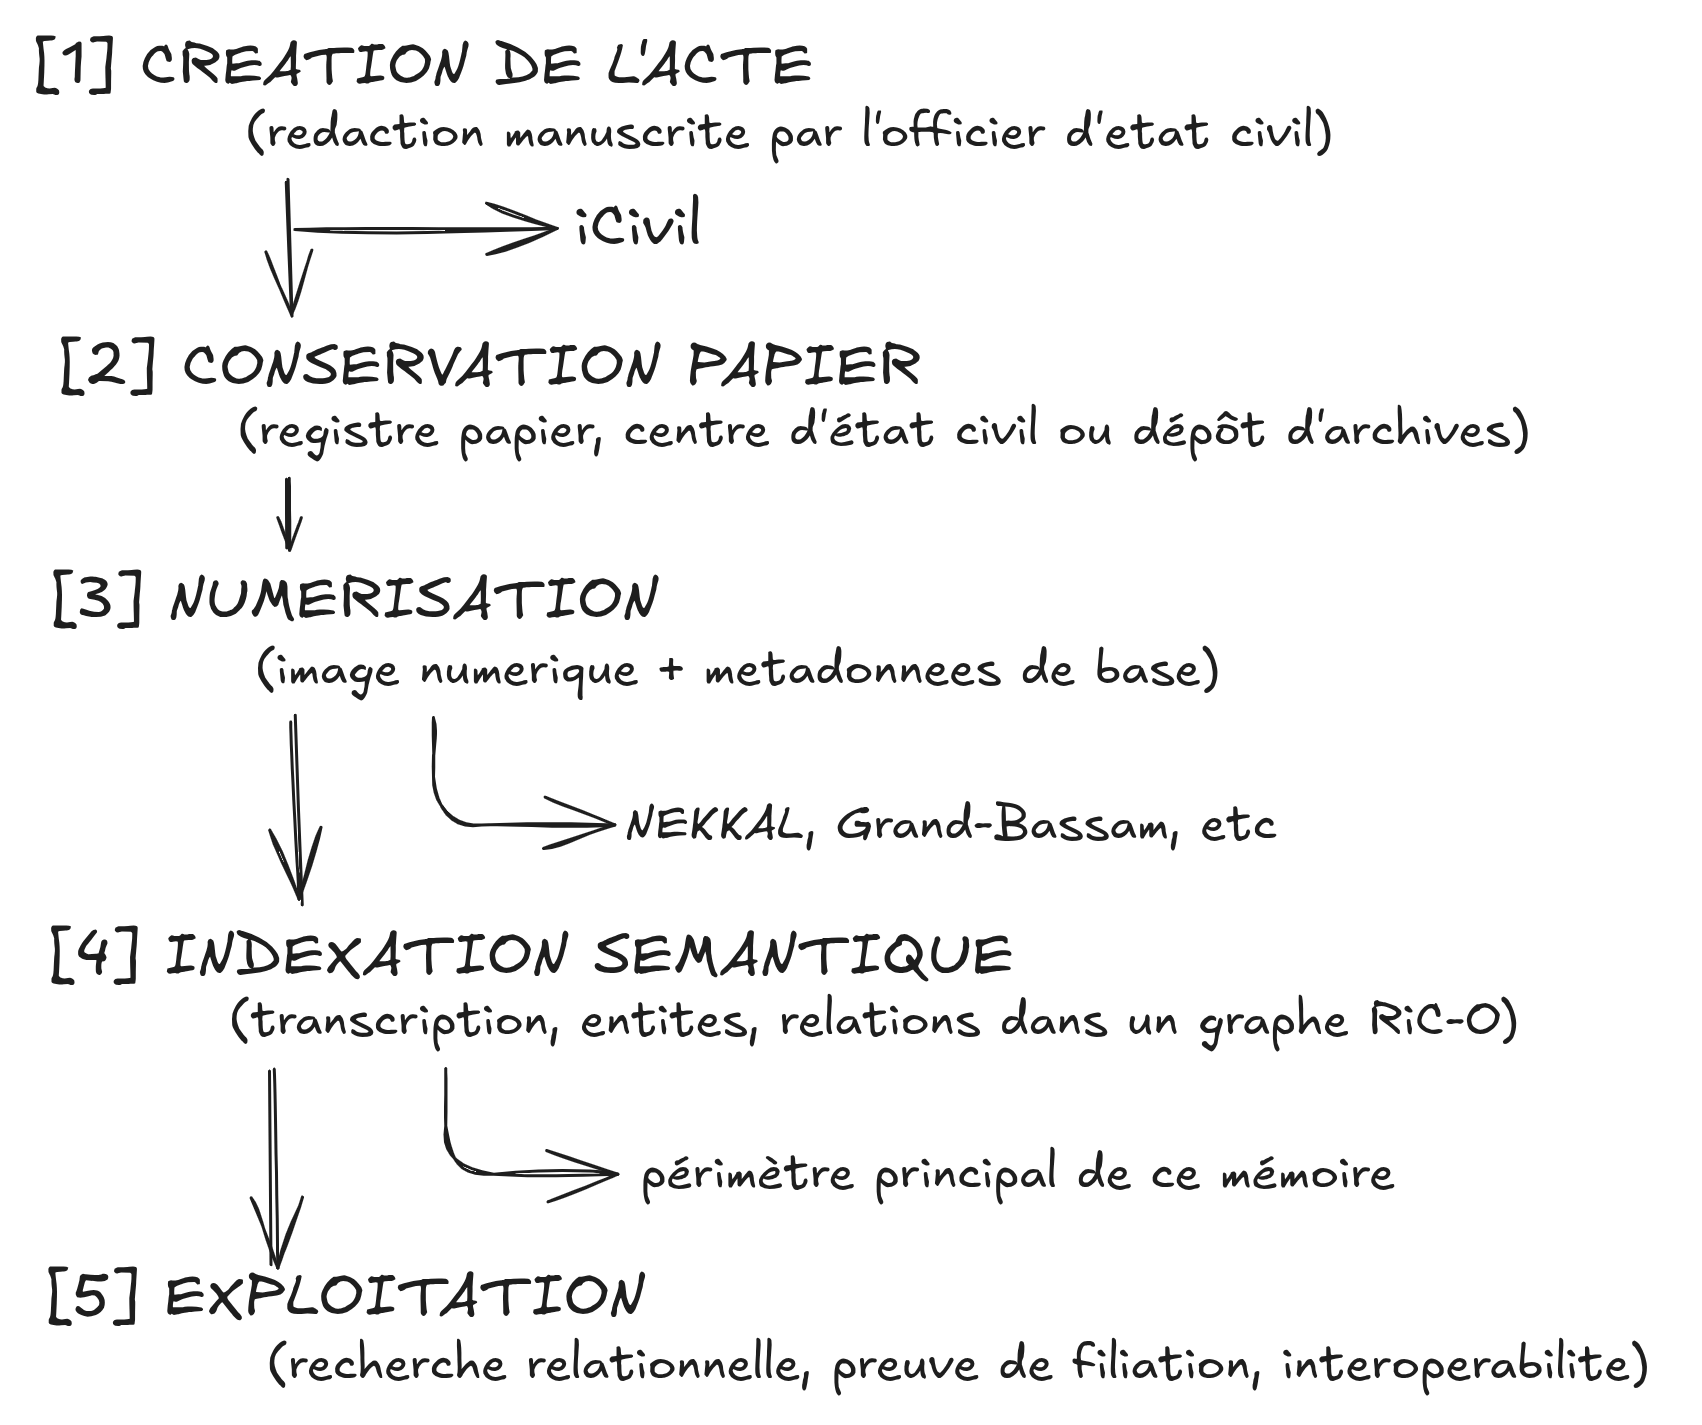
\includegraphics[width=0.8\textwidth]{figures/représentation_cycle_de_vie_acte.png}
    \caption{Cycle de vie de l'acte d'État civil et couverture des reformes actuelles. \textit{Source : l'auteur, réalisé avec Excalidraw}}
    \label{fig:lifecycle_of_registers}
\end{figure}

Ces deux démarches illustrent des modalités distinctes de déploiement progressif : expérimentation locale préalable à une éventuelle extension nationale dans le cas ivoirien, et projet de collecte et de conversion numérique à périmètre national dans le cas congolais.
Les sources consultées ne documentent toutefois pas de représentation sémantique des liens entre personnes et événements.
Le présent mémoire examine précisément la faisabilité d'une telle structuration pour les registres manuscrits.

Au Cameroun, la loi n\textsuperscript{o}~2024/001 du 24 juillet 2024 régissant les archives fixe un cadre général pour la gestion, la conservation, la sécurisation et la modernisation des archives \cite{cameroun2024loiarchives}.
Elle ne définit toutefois pas de chaîne opérationnelle spécifique de transcription, de résolution d'entités ou d'indexation sémantique des registres d'état civil manuscrits.
Ce mémoire examine précisément les conditions techniques et méthodologiques d'une telle exploitation.

Comme l'illustre la Figure~\ref{fig:lifecycle_of_registers}, les réformes examinées couvrent principalement l'enregistrement numérique, la numérisation et, dans certains cas, l'indexation documentaire.
Les sources publiques consultées ne décrivent pas de dispositif d'indexation sémantique reliant explicitement personnes, événements et actes.
Le mémoire se situe à ce niveau, en évaluant la transformation de registres manuscrits en données relationnelles, traçables et interrogeables.

\section{Les registres manuscrits d'état civil comme patrimoine documentaire}

Cette section examine les registres manuscrits comme objets matériels, administratifs et probatoires.
Leur état de conservation conditionne directement la qualité des images produites lors de la numérisation et, par conséquent, les performances des outils de reconnaissance automatique examinés en section 1.4.

\subsection{Diversité matérielle, scripturaire et enjeux de conservation}

Les registres d'état civil peuvent présenter des formats, supports, encres, écritures et formulaires variables selon les périodes et les lieux de production.
Les études consacrées aux manuscrits d'Afrique subsaharienne documentent des difficultés comparables de conservation, liées à la variabilité des supports et à leur vulnérabilité environnementale \cite{abdoulahi2019contribution,ala2005batiments}.
Ce rapprochement relève toutefois d'une analogie matérielle : les corpus diffèrent par leur fonction, leur langue et leurs conditions de production.

\begin{figure}[H]
    \centering
    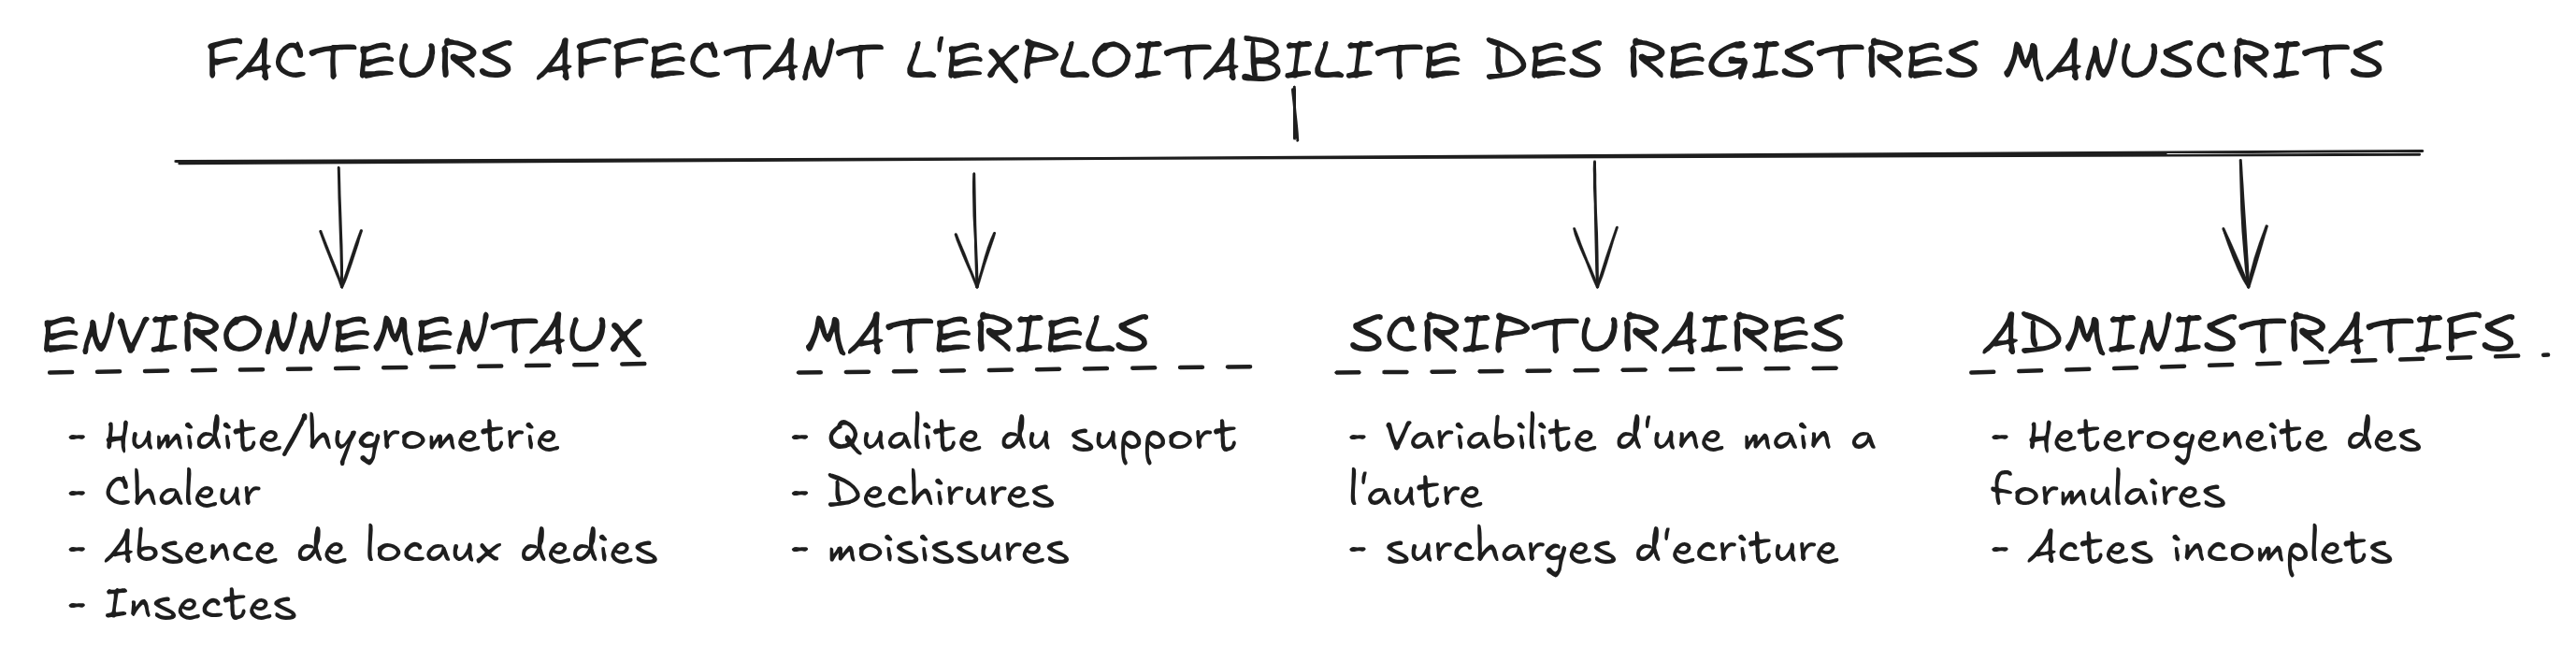
\includegraphics[width=0.99\textwidth]{figures/facteurs-exploitabilite.png}
    \caption{Facteurs affectant l'exploitabilité des registres manuscrits. \textit{Source : l'auteur, réalisé avec Excalidraw}}
    \label{fig:facteurs-exploitabilite}
\end{figure}

Dans les contextes où les conditions de conservation ne sont pas régulées, la température, l'humidité, les moisissures, les insectes et les manipulations répétées peuvent dégrader le papier et les encres.
Ces facteurs affectent la lisibilité des actes et augmentent la difficulté de leur transcription automatique.
Ils imposent donc de documenter, pour chaque corpus, l'état matériel des registres afin d'interpréter les résultats de reconnaissance et d'extraction.
La dégradation physique n'annule pas la valeur probatoire de l'acte, mais elle peut limiter son accessibilité et son exploitabilité.
La Figure~\ref{fig:facteurs-exploitabilite} synthétise les facteurs susceptibles d'affecter l'exploitabilité des registres.

\subsection{Valeur probatoire des actes anciens et préservation numérique en contexte de ressources limitées}

Les actes d'état civil anciens peuvent conserver une valeur probatoire durable lorsqu'ils restent authentifiables, intègres et rattachables à une autorité compétente.
Ils constituent des preuves importantes de l'identité juridique, de l'âge ou de la filiation, notamment en l'absence de documents contemporains \parencite{uneca2020status,un2023guidelines}.

La numérisation améliore l'accès aux registres fragiles, mais ne remplace ni leur conservation physique ni leur valeur juridique.
Les travaux consacrés à la préservation numérique dans les bibliothèques universitaires sud-africaines mettent notamment en évidence des difficultés de financement pérenne, de compétences spécialisées, d'obsolescence technologique et d'infrastructure \parencite{masenyaFactorsThatInfluence2020,masenyaDigitalPreservationPractices2019}.
Ces résultats fournissent un point de comparaison utile pour les institutions archivistiques disposant de ressources limitées, sans pouvoir être généralisés mécaniquement à tous les services d'état civil.

Dans cette perspective, la numérisation doit être distinguée de l'exploitation sémantique.
Le graphe de connaissances doit donc être conçu comme une couche sémantique dérivée, traçable et explicitement reliée aux actes sources.
L'enjeu n'est pas de remplacer l'acte original, mais d'en améliorer l'exploitabilité sans produire d'assertions non attestées.

\section{Standards et modèles de description archivistique}

Le choix d’un modèle de représentation adapté aux relations présentes dans les actes d’état civil suppose de distinguer les fonctions de préservation, de description hiérarchique et de description sémantique.
Cette section examine les principaux standards mobilisables avant de présenter RiC-O, retenu comme cadre de modélisation dans ce mémoire.

\subsection{Modèles classiques : OAIS, EAD et Dublin Core}

Le modèle OAIS (\textit{Open Archival Information System}), normalisé par l’ISO 14721, constitue un cadre de référence pour la préservation numérique.
Il décrit les fonctions d’un système d’archivage --- versement, stockage, gestion des données, administration, planification de la préservation et accès --- ainsi que les paquets d’information qui circulent entre elles.
OAIS éclaire donc l’organisation nécessaire à la conservation durable des archives, sans définir la représentation sémantique du contenu d'un document : il ne dit rien de la manière de représenter un acte de naissance et les personnes qu'il met en relation.
Sa pertinence pour ce mémoire est donc réelle mais indirecte —-- il éclaire les fonctions que devra assumer l'infrastructure de conservation, sans se substituer à un modèle sémantique du contenu.

EAD (\textit{Encoded Archival Description}) est un standard XML destiné à l’encodage des instruments de recherche archivistiques.
Il permet de décrire un fonds à plusieurs niveaux, du fonds à la pièce, selon une organisation généralement hiérarchique.
Il peut ainsi situer un acte dans son contexte de production et conserver des informations descriptives à son sujet.
Toutefois, EAD ne fournit pas, à lui seul, un modèle explicite d’entités persistantes permettant de relier, à travers plusieurs actes, un officier d’état civil, un déclarant, un enfant, des parents ou un événement selon des relations sémantiques typées.

Dublin Core propose un vocabulaire générique de métadonnées destiné à la découverte et à l’échange de ressources hétérogènes.
Dans sa version simple, il repose sur quinze éléments tels que le titre, le créateur, le sujet ou la date.
Ce niveau de généralité facilite l’interopérabilité minimale, mais demeure insuffisant pour distinguer systématiquement les rôles spécifiques intervenant dans un acte d’état civil.
Une propriété comme \texttt{creator} peut désigner une personne ou une organisation responsable de la ressource, sans exprimer nécessairement la fonction précise exercée dans l’acte.

Pris isolément, OAIS, EAD et Dublin Core répondent donc à des besoins complémentaires : préservation du système, description hiérarchique des fonds et découverte de ressources.
Ils ne fournissent toutefois pas un modèle archivistique complet permettant de représenter explicitement les relations entre les personnes, les événements et les actes d’état civil.
Cette limite motive l’étude d’une approche fondée sur RiC-O.

\subsection{Records in Contexts et l’ontologie RiC-O : principes, structure et interopérabilité}

Développé par le Groupe d’experts en description archivistique (EGAD) du Conseil international des archives depuis 2012, le standard \textit{Records in Contexts} (RiC) a été conçu comme un successeur des quatre normes descriptives antérieures de l’ICA : ISAD(G), ISAAR(CPF), ISDF et ISDIAH.
Il vise à les articuler dans un cadre conceptuel commun, centré sur les entités archivistiques et leurs contextes plutôt que sur des descriptions produites séparément.

RiC comporte quatre parties complémentaires : les fondements de la description archivistique (RiC-FAD), le modèle conceptuel (RiC-CM), l’ontologie (RiC-O) et les lignes directrices d’application (RiC-AG).
Les versions 1.0 de RiC-FAD, RiC-CM et RiC-O ont été publiées fin 2023 ; RiC-AG demeure en cours d’élaboration \textbf{ica2023ricrelease,ica2025ricwebinar}.
RiC-O, dans sa version 1.1, est une ontologie OWL 2 qui formalise RiC-CM et fournit un vocabulaire ainsi que des règles formelles pour produire des jeux de données RDF décrivant des ressources archivistiques et leurs contextes \parencite{icaegad2025rico11,clavaudica}.

L’apport de RiC-O tient à sa modélisation orientée entités-relations.
Documents, agents, lieux, événements, activités et règles de gestion peuvent être représentés comme des entités distinctes et reliés au moyen de propriétés explicites.
Un acte de naissance peut ainsi être décrit à la fois comme une ressource archivistique, comme la trace d’un événement et comme un document associé à plusieurs agents exerçant des rôles différents.
Cette approche ne résout pas automatiquement l’identification des personnes ni l’extraction du contenu manuscrit ; elle fournit le cadre nécessaire pour représenter, documenter et interroger les relations établies à partir des actes.

Les jeux de données produits en RDF peuvent être reliés à d’autres vocabulaires et référentiels, puis interrogés au moyen de SPARQL lorsqu’ils sont stockés dans une infrastructure compatible.
L’interopérabilité effective dépend toutefois des choix de modélisation, de la stabilité des identifiants, des règles de transformation, de la provenance des assertions et de la gouvernance des données.
RiC-O constitue ainsi un cadre de référence, non une solution technique complète de peuplement ou d’exploitation d’un graphe.

\subsection{Profils d’application RiC-O : état des lieux}

RiC-O est une ontologie générique : son application à un domaine particulier suppose de sélectionner les classes et propriétés pertinentes, de définir des contraintes d’usage et, si nécessaire, de documenter des extensions.
Les futures lignes directrices RiC-AG ont précisément vocation à fournir aux professionnels et aux développeurs des recommandations et des exemples de mise en œuvre de RiC-CM et RiC-O \textbf{ica2023ricfad}.

Les démonstrations actuellement disponibles portent principalement sur la conversion ou l’exploitation de métadonnées archivistiques existantes, notamment issues d’EAD, d’EAC-CPF ou de METS.
Elles ne constituent pas nécessairement des profils de production applicables tels quels à l’état civil.
Dans les ressources consultées, aucun profil RiC-O spécifiquement consacré aux registres d’état civil manuscrits, et a fortiori aux corpus d’Afrique subsaharienne, n’a été identifié.

Cette lacune ne signifie pas que le domaine est absent de RiC-O : le standard fournit des mécanismes génériques pour représenter des documents, agents, événements, lieux et relations.
Elle indique plutôt que les règles d’application propres à l’état civil --- modélisation de la filiation, distinction des rôles, gestion des actes associés, traitement des informations incertaines et provenance des assertions --- restent à définir et à évaluer.
C’est dans cet espace que s’inscrit l’objectif scientifique OS2 du mémoire.

